\section{Argument Schemes for Goal Modeling (GMAS)}
\label{sect:gmas}

In this section we develop a set of argument schemes and critical questions for goal modeling. The list of argument schemes and critical questions is shown in table~\ref{table:argument-schemes}. The first four argument schemes (AS0-AS4) are argument for an element of a goal model, the next seven (AS5-AS11) are about relationships, and the remain two (AS12-AS13) are about intentional elements in general. For each critical question, the right column shows the effect of answering the critical questions affirmatively, which can be DISABLE (disable the element of the original argument), INTRO (introduce a new element and argument), or REPLACE (replace the element of the original argument). For instance, if the critical question CQ0 ``Is the actor relevant?'' is answered with ``No'', then the actor of the original argument AS0 will be disabled in the goal model. We come back to these effects in more detail in subsection~\ref{sect:?} of this section.

We obtained the list in table~\ref{table:argument-schemes} by analyzing transcripts of discussions between students about the development of an information system. In this section, we provide details of this analysis process with concrete examples.

\begin{table*}[h]
\centering
\begin{tabularx}{\textwidth}{|l|l|l|X|l|l|}
\hline
\multicolumn{2}{|c|}{\textbf{Argument scheme}} & \multicolumn{2}{c|}{\textbf{Critical Questions}} & \textbf{Effect}\\
\hline
AS0 & Actor $a$ is relevant & CQ0 &Is the actor relevant? & DISABLE\\
\hline
AS1 & Actor $a$ has resource $R$ & CQ1 &Is the resource available? & DISABLE\\
\hline
AS2 & Actor $a$ can perform task $T$ & CQ2 &Is the task possible? & DISABLE\\
\hline
AS3 & Actor $a$ has goal $G$ & CQ3 & Can the desired goal be realized? & DISABLE\\
\hline
AS4 & Actor $a$ has softgoal $S$ & CQ4 & Is the softgoal a legitimate softgoal?& DISABLE\\
\hline
\hline
AS5 & goal $G$ decomposes into tasks $T_1,\ldots,T_n$ & CQ5a & Does the goal decompose into the tasks?& DISABLE\\
& & CQ5b & Does the goal decompose into any other tasks?& INTRO\\
\hline
AS6 & Task $T$ contributes to softgoal $S$& CQ6a & Does the task contribute to the softgoal?& DISABLE\\
&& CQ6b & Are there alternative ways of contributing to the same softgoal?& INTRO \\
&& CQ6c & Does the task have a side effect which contribute negatively to some other softgoal?& INTRO\\
&& CQ6d & Does the task contribute to some other softgoal?& INTRO\\
\hline
AS7 & Goal $G$ contributes to softgoal $S$ & CQ7a & Does the goal contribute to the softgoal?& DISABLE\\
&& CQ7b & Does the goal contribute to some other softgoal?& INTRO\\
\hline
AS8 & Resource $R$ contributes to task $T$ & CQ8 & Is the resource required in order to perform the task?& DISABLE\\
\hline
AS9 & Actor $a$ depends on actor $b$ & CQ9 & Does the actor depend on any actors?& INTRO\\
\hline
AS10 & Task $T_1$ decomposes into tasks $T_2,\ldots,T_n$ & CQ10a & Does the task decompose into other tasks?& INTRO\\
 &  & CQ10b & Is the decomposition type correct? (AND/OR/XOR)& REPLACE\\
\hline
AS11 & Task $T$ contributes negatively to softgoal $S$& CQ11 & Does the task contribute negatively to the softgoal?& DISABLE\\
\hline
\hline
AS12 & Element $IE$ is relevant & CQ12a & Is the element relevant? & DISABLE\\
&  & CQ12b & Is the element redundant? & DISABLE\\
\hline
AS13 & Element $IE$ has name $n$ & CQ12a & Is the name clear? & REPLACE\\
&  & CQ12b & Is the name ambiguous? & REPLACE\\
\hline
\end{tabularx}
\caption{List of argument schemes (AS0-AS13, left column), critical questions (CQ0-CQ12, middle column), and the effect of answering them (right column).}
\label{table:argument-schemes}
\end{table*}

\subsection{Details experiment}

The transcripts we used are created as part of two master theses on improving design reasoning~\cite{masterthesis1,masterthesis2}.

\paragraph{Subjects} The subjects for the case study are three teams of Master students from the University of Utrecht, following a Software Architecture course. Two teams consist of three students, and one team consists of two students.

\paragraph{Experimental Setup} The assignment used for the experiments is to design a traffic simulator. Designers are provided a problem description, requirements, and a description of the desired outcomes. The original version of the problem descrption~\cite{UCIworkshop} is well known in the field of design reasoning since it has been used in a workshop\footnote{\url{http://www.ics.uci.edu/design-workshop/}}, and transcripts of this workshop have been analyzed in detail~\cite{Petre:2013:SDA:2535028}. Although the concepts of traffic lights, lanes, and intersections are common and appear to be simple, building a traffic simulator to represent these relationships and events in real time turns out to be challenging. Participants were asked to use a think-aloud method during the design session. For the student groups the assignment was slightly adjusted to include several viewpoints as end products in order to conform to the course material~\cite{Bass:2012:SAP:2392670}. The final problem descriptions can be found in Appendix A of Schriek's master thesis~\cite{masterthesis1}. All groups were instructed to apply the \emph{functional architecture method}, focusing on developing the \emph{context}, the \emph{functional}, and the \emph{informational} viewpoints of the traffic simulator software. The students had two hours for the tasks, and the transcripts document the entire discussion. The details of the transcripts are shown in table~\ref{table:transcripts:info}.

\begin{table}[ht]
\centering
\begin{tabular}{|l|l|l|l|}
\hline
& transcript $t_1$ & transcript $t_2$ & transcript $t_3$\\
\hline
participants & 2 & 3 & 3\\
\hline
duration & 1h34m52s & 1h13m39s & 1h17m20s\\
\hline
\end{tabular}
\caption{Number of participants and duration of the transcripts.}
\label{table:transcripts:info}
\end{table}

\paragraph{Annotation method} 

We started with an initial list of 10 argument schemes and 18 critical questions that we derived from PRAS. We annotated transcripts with the arguments and critical questions from this list. If we found arguments or critical questions that did not appear in the original list, we added them and counted them as well. Argument schemes that did not appear were removed from the list. Most of the occurrences were not literally found back, but had to be inferred from the context. This can be seen in the various examples we will discuss.

It is generally known in the argumentation literature that it can be very difficult to annotate arguments correctly.\todo{Marc}{Floris}{add citation} Arguments are often imprecise, lack conclusion, and may be supported by non verbal communication that is not captured in the transcripts. Still, since research on argument extraction in the requirement engineering domains is in its infancy, we believe that our evaluation is useful by itself. Furthermore, our annotation is openly available\footnote{\todo{Marc}{Marc}{provide url}}, we provide parts of our annotation in Appendix~\ref{sect:transcripts:excerpts}, and most of the examples from this article come from the transcripts. In this way, we aim to make our annotation process as transparent as possible.

\paragraph{Results}

We found a total of 120 instantiations of the existing argument schemes AS0-AS9 in the transcripts. The most used argument scheme was AS2: ``Actor $A$ has task $T$'', but each argument scheme has been found back in the transcripts at least twice (table~\ref{table:transcripts:results:argumentschemes}). 

Of our critical questions, we annotated 9 instantiations. Example of critical questions are CQ0, questioning the relevance of an actor (table~\ref{table:transcript:as0-cq0}) and CQ2, questioning the possibility of a task (table~\ref{table:transcript:as2-cq_star_1-cq2}).

\begin{table}[ht]
\centering
\begin{tabularx}{0.5\textwidth}{|l|X|l|l|l|>{\bfseries}l|}
\hline
\multicolumn{2}{|c|}{\textbf{Scheme/Question}} & $t_1$ & $t_2$ & $t_3$ & \textbf{total}\\
\hline 
AS0 & Actor & 2 & 2 & 5 & 9\\
\hline
AS1 & Resource & 2 & 4 & 5 & 11\\
\hline
AS2 & Task/action & 20 & 21 & 17 & 58\\
\hline
AS3 & Goal & 0 & 2 & 2 & 4\\
\hline
AS4 & Softgoal & 3 & 4 & 2 & 9\\
\hline
AS5 & Goal decomposes into tasks & 4 &0& 4 & 8\\
\hline
AS6 & Task contributes to softgoal & 6 & 2 &0& 8\\
\hline
AS7 & Goal contributes to softgoal &0& 1 & 1 & 2\\
\hline
AS8 & Resource contributes to task & 0 & 4 & 3 & 7\\
\hline
AS9 & Actor depends on actor &0& 1 & 3 & 4\\
\hline
AS10 & Task decomposes into tasks & 11 &14 &11 &36\\ 
\hline
AS11 & Task contributes negatively to softgoal & 2 & 1 & 0 & 3\\
\hline
\hline
CQ2 & Task is possible? & 2 & 2 & 1 & 5\\
\hline		
CQ5a & Does the goal decompose into the tasks? & 0 & 1 & 0 & 1\\
\hline
CQ5b & Alternative ways to realize goal? & 1 & 0 & 0 & 1\\
\hline
CQ6b & Task has negative side effects? & 2 & 0 & 0 & 2\\
\hline
CQ10a & Task decompose into other tasks? & 1 &2 &0&3\\
\hline
CQ10b & Decomposition type correct? &1 &0& 1 &2\\
\hline
\hline
CQ12 & Useless/irrelevant/redundant element & 2 & 3 & 2 &7\\
\hline
CQ13 & Clarifying an element &3 &10 & 3 & 16\\
\hline
\hline
\multicolumn{2}{|c|}{\textbf{TOTAL}}&69&80&69&218\\
\hline
\end{tabularx}
\caption{Number of occurrences of AS0-AS9, CQ0-CQ12 in the transcripts. Critical questions not appearing in this table were not found back in the transcripts.}
\label{table:transcripts:results:argumentschemes}
\end{table}

We found that answering a critical questions can have three effects on the original argument:
\begin{itemize}
\item \emph{INTRO}: Introduce a new element with a corresponding argument. This operation does not attack the original argument, but rather creates a new argument.
\item \emph{DISABLE:} Disable the element of the argument scheme to which the critical questions pertains. This operation does not create a new argument, but only disables (i.e., attacks) the original one.
\item \emph{REPLACE:} Replace the element of the argument scheme with a new element. This operation both introduces a new argument and attacks the original one.
\end{itemize}

\subsection{Analysis}

The analysis of the results of our empirical evaluation consists of three parts. First, we analyze the argument schemes, then the critical questions, and finally we analyze the effect of answering a critical question affirmatively.

\paragraph{Analysis of the argument schemes}
Our initial list of argument schemes consists of AS1-AS4, AS5-AS9 (figure~\ref{table:argument-schemes}). Therefore, the difference between the initial list of argument schemes and those found back in the transcripts is quite small. We found it surprising that we were able to find back all the schemes in the transcript at least twice, even more since the topic of discussion wasn't goal models, but more generally the architecture of an information system. This gives us an indication that these argument schemes are able to capture arguments used in those type of discussions to some extent. 

More generally, we observed that our initial list is rather limited, which is a consequence of the fact that it is derived from PRAS. Since PRAS only considers very specific types of relationships, we are not able to capture many other relationships existing in GRL. GRL has four types of intentional elements (softgoal, goal, task, resource) and four types of relationships (positive contribution, negative contribution\footnote{In fact, a contribution can be any integer in the domain [-100,100], but for the sake of simplicity we only consider two kinds of contributions here.}, dependency, decomposition), allowing theoretically $4^3=64$ different types of argument schemes, of which we currently only consider 11. Our analysis however shows that many of these schemes are not often used, and thus gives us some confidence in the resulting list.

\paragraph{Analysis of the critical questions} The difference between the initial list of critical questions and those we found back in the transcripts is much larger than for the critical questions. On the one hand, we found back few of the critical questions we initially proposed. However, this does not mean that they weren't implicitly used in the minds of the participants. If a participants makes an argument for a contribution from a task to a softgoal, it may very well be that she was asking herself the question ``Does the task contribute to some other softgoal?''. However, many of these critical questions are not mentioned explicitly. If we assume this explanation is at least partially correct, then this would mean that critical questions may still play a role when formalizing the discussions leading up to a goal model, and it would be limiting to leave them out of our framework. In the context of tool support, we believe that having these critical questions available may stimulate discussions.

\subsection{Examples}

For each transcript, we manually create a GRL model from the argument schemes and critical questions we found in them, in order to verify whether the arguments put forward by the participants were sufficiently informative. An example of such a model is shown in figure~\ref{fig:transcripts:grl}. We added green and red dots to various elements and relationships in the figure. A green dot indicates there is an underlying argument for the element that is accepted, while a red dot indicates a rejected underlying argument. Note that if the underlying argument is rejected, the corresponding GRL element has been disabled. Some elements do not have a corresponding green or red dot. In that case, we have inferred the elements from the discussion, but we could not explicitly find back arguments for it.

We now discuss various instantiations of argument schemes and the result of answering critical questions in more detail. The examples below come from all three transcripts, and therefore not always correspond to the goal model in figure~\ref{fig:transcripts:grl}. For each example we provide transcript excerpts, a visualization of the arguments, and the corresponding goal model elements.

\subsubsection{Irrelevant actor}

The transcript excerpt of the first example is shown in table~\ref{table:transcript:irrelevant-actor} in the appendix. It consists of participant P1 putting forth the suggestion to include actor \emph{Development team} into the model. This is then questioned by person P2, who argues that the professor will develop the software, so there won't be any development team. 

We formalized the first statement as an instantiation of argument scheme AS0: \emph{Actor development team is relevant}. This argument is then attacked by answering critical question CQ0: \emph{Is actor development team relevant?} with \emph{No}. This results in two arguments, AS0 and CQ0, where CQ0 attacks AS0. This is shown in figure~\ref{fig:examples:relevant-actor:arguments}.

Argument scheme AS0 is an argument to include actor \emph{Development team} into the GRL model. Therefore, by attacking it the argument is no longer accepted, and as a result the actor is disabled in the resulting GRL model (figure~\ref{fig:examples:relevant-actor:grl}). Note we added a red traceability link from the rejected argument to the disabled GRL element.

\begin{figure}[ht!]
\centering
\begin{subfigure}[b]{0.22\textwidth}
        \centering
        \begin{tikzpicture}[->]
        \node (a0) [shape=rectangle, draw=black!60, text=black!40] at (0,0) {
            \begin{tabularx}{\textwidth}{X}
                \textbf{(AS0)} Development team is relevant 
            \end{tabularx}
        } ;
        \node (a1) [shape=rectangle,draw] at (0,-2){
            \begin{tabularx}{\textwidth}{X}
                \textbf{(CQ0)} Development team is not relevant (\emph{The professor makes the software})
            \end{tabularx}
        };
        \node[circle,draw=black, fill=red, inner sep=0pt,minimum size=8pt] (trace) at (1.2,-0.3) {};
        
         \path[line width=1mm]
    (a1) edge[draw=black] (a0);
\end{tikzpicture}
        \caption{Arguments}
        \label{fig:examples:relevant-actor:arguments}
    \end{subfigure}\hfill
    \begin{subfigure}[b]{0.22\textwidth}
        \centering
        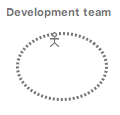
\includegraphics[width=\textwidth]{img/actor_disabled}
        \caption{GRL elements}
        \label{fig:examples:relevant-actor:grl}
    \end{subfigure}
\caption{Argument schemes and critical questions (left) and GRL model (right) of a discussion about the relevance of actor Development team.}
\label{fig:examples:relevant-actor}
\end{figure}

We see from this example that answering critical question CQ0 affirmatively has the effect of disabling the corresponding actor \emph{Development team}. Therefore, critical question CQ0 has the associated effect DISABLE in table~\ref{table:argument-schemes}.

\begin{figure*}[h]
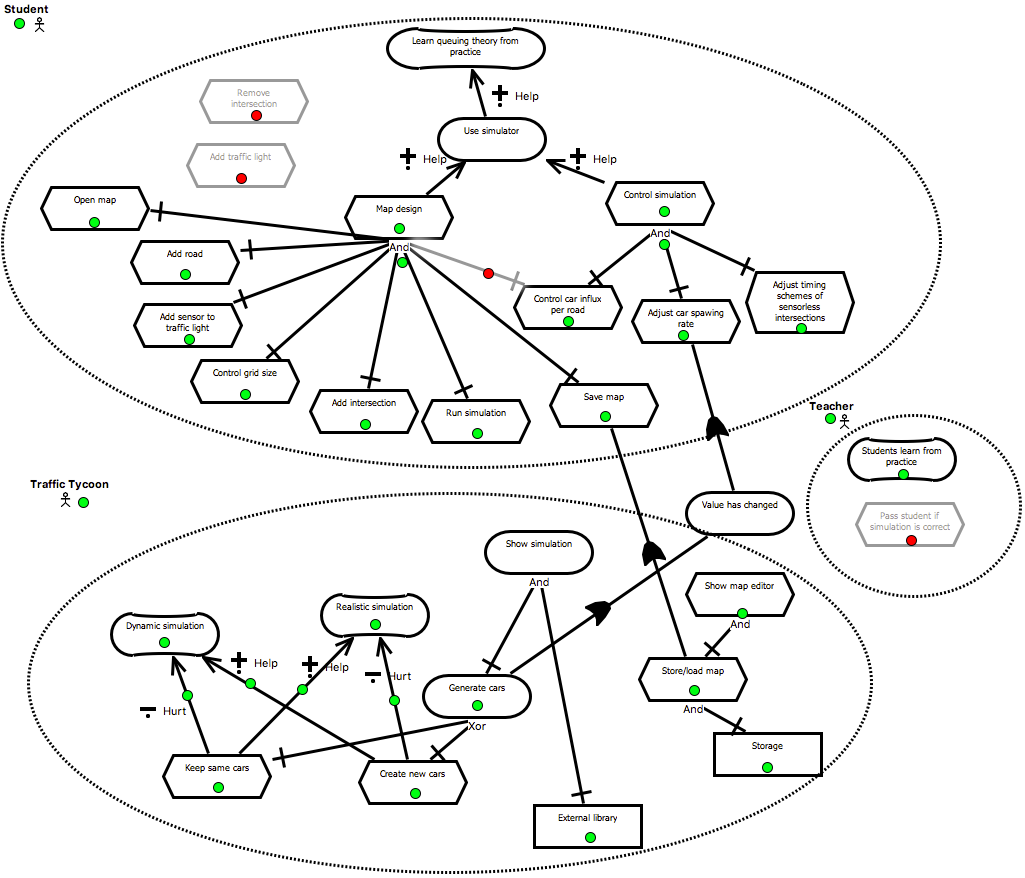
\includegraphics[width=\textwidth]{img/transcript_grl}
\caption{The GRL model manually constructed from transcript 1. Green dots indicate accepted underlying arguments, red dots indicate rejected underlying arguments. Elements and relationships with no dot have been inferred by us.}
\label{fig:transcripts:grl}
\end{figure*}